\documentclass[tikz,border=6pt]{standalone}
\usepackage{amsmath}
\usepackage{pgfplots}
\pgfplotsset{compat=1.18}

% Data: choose simple 1D points
% Class +1 : x < 1  and  x > 2
% Class -1 : 1 < x < 2
% Mapping phi(x) = (x, x^2). In (X,Y)=(x, x^2), the separator is linear: Y - 3X + 2 = 0.

\begin{document}
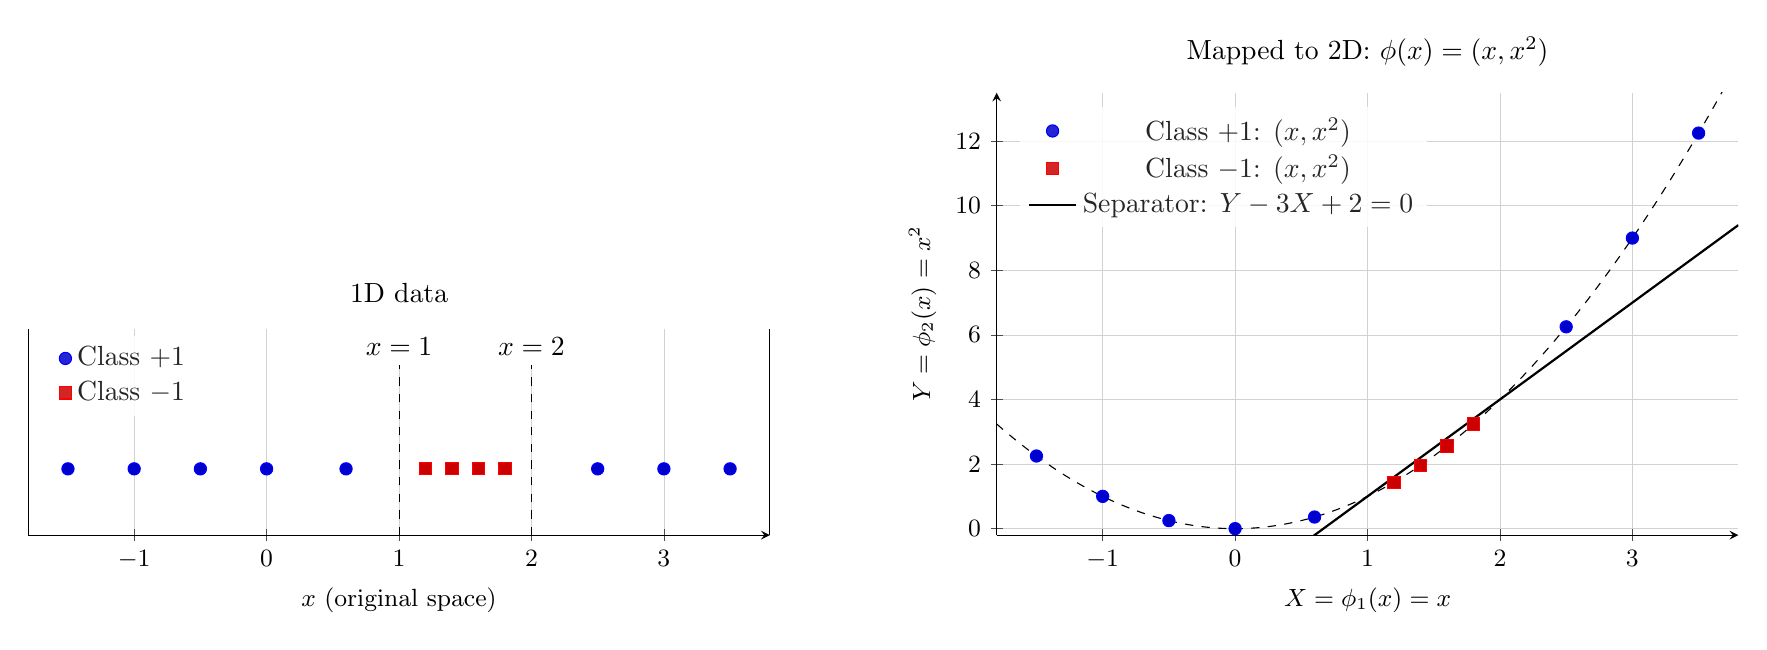
\begin{tikzpicture}

% -------- LEFT: 1D original space --------
\begin{axis}[
  width=11cm, height=4.2cm,
  at={(0,0)},
  axis x line=bottom,
%   axis y line=left,
  ymin=-0.2, ymax=1.2,
  xmin=-1.8, xmax=3.8,
  ytick=\empty,
  xlabel={$x$ (original space)},
  title={1D data},
  grid=both, grid style={line width=.1pt, draw=gray!20},
  major grid style={line width=.2pt, draw=gray!35},
  tick style={black!70},
  label style={font=\small},
  tick label style={font=\small},
  legend style={draw=none, fill=white, fill opacity=0.85},
  legend pos=north west
]

  % Class +1 points: x < 1 and x > 2
  \addplot+[only marks, mark=*, mark size=2.2pt] coordinates
    {(-1.5,0.25) (-1.0,0.25) (-0.5,0.25) (0.0,0.25) (0.6,0.25) (2.5,0.25) (3.0,0.25) (3.5,0.25)};
  \addlegendentry{Class $+1$}

  % Class -1 points: 1 < x < 2
  \addplot+[only marks, mark=square*, mark size=2.2pt] coordinates
    {(1.2,0.25) (1.4,0.25) (1.6,0.25) (1.8,0.25)};
  \addlegendentry{Class $-1$}

  % Vertical guides at x=1 and x=2
  \addplot[very thin, dashed] coordinates {(1,-0.2) (1,1.2)};
  \node[anchor=south,fill=white] at (axis cs:1,0.95) {$x=1$};

  \addplot[very thin, dashed] coordinates {(2,-0.2) (2,1.2)};
  \node[anchor=south,fill=white] at (axis cs:2,0.95) {$x=2$};

\end{axis}

% -------- RIGHT: 2D feature space (x, x^2) --------
\begin{axis}[
  width=11cm, height=7.2cm,
  at={(12.3cm,0)},
  axis x line=bottom,
  axis y line=left,
  xmin=-1.8, xmax=3.8,
  ymin=-0.2, ymax=13.5,
  xlabel={$X=\phi_1(x)=x$},
  ylabel={$Y=\phi_2(x)=x^2$},
  title={Mapped to 2D: $\phi(x)=(x, x^2)$},
  grid=both, grid style={line width=.1pt, draw=gray!20},
  major grid style={line width=.2pt, draw=gray!35},
  tick style={black!70},
  label style={font=\small},
  tick label style={font=\small},
  legend style={draw=none, fill=white, fill opacity=0.85},
  legend pos=north west
]

  % Class +1 mapped points: (x, x^2)
  \addplot+[only marks, mark=*, mark size=2.2pt] coordinates
    {(-1.5,2.25) (-1.0,1.00) (-0.5,0.25) (0.0,0.00) (0.6,0.36) (2.5,6.25) (3.0,9.00) (3.5,12.25)};
  \addlegendentry{Class $+1$: $(x,x^2)$}

  % Class -1 mapped points: (x, x^2)
  \addplot+[only marks, mark=square*, mark size=2.2pt] coordinates
    {(1.2,1.44) (1.4,1.96) (1.6,2.56) (1.8,3.24)};
  \addlegendentry{Class $-1$: $(x,x^2)$}

  % Linear separator in (X,Y): Y - 3X + 2 = 0  => Y = 3X - 2
  \addplot[domain=-1.8:3.8, samples=2, thick] {3*x - 2};
  \addplot[domain=-1.8:3.8, samples=300, dashed] {x*x};
  \addlegendentry{Separator: $Y-3X+2=0$}

  % Optional labels for the two sides (visual cue)
%   \node[anchor=west] at (axis cs:-1.7,0.6) {Class $+1$};
%   \node[anchor=west] at (axis cs:1.1,2.8) {Class $-1$};
%   \node[anchor=west] at (axis cs:2.6,9.5) {Class $+1$};

\end{axis}

\end{tikzpicture}
\end{document}